\item Prism 1 of mass \(m_1\) and with angle \(\alpha\) (see Fig. 1.23) rests on a horizontal surface. Bar 2 of mass \(m_2\) is placed on the prism. Assuming the friction to be negligible, find the acceleration of the prism. 
    \begin{center}
        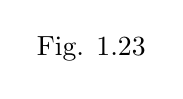
\begin{tikzpicture}
            \node at (0, 0) {Fig. 1.23};
        \end{tikzpicture}
    \end{center}\begin{solution}
    \begin{center}
        \begin{tikzpicture}
            \pic at (0, 0) {frame=3cm};
        \end{tikzpicture}
    \end{center}
    
    \begin{align*}
        \intertext{Let us draw the force diagram of each body, and on this basis we observe that the prism moves towards right (say) with an acceleration $\vec{w}_1$ and the bar 2 of mass $m_2$ moves down the plane with respect to 1, say with acceleration $\vec{w}_{21}$, then}
        \vec{w}_2 &= \vec{w}_{21} + \vec{w}_1 \quad \text{(see figure).}
        \intertext{Let us write Newton’s second law of both bodies in projection form along positive $y_2$ and $x_1$ axes as shown in the figure.}
        m_2 g \cos \alpha - N &= m_2 w_{2(y_2)} = m_2 [w_{21(y_2)} + w_{1(y_2)}] = m_2 [0 + w_1 \sin \alpha]
        \intertext{or}
        m_2 g \cos \alpha - N &= m_2 w_1 \sin \alpha \tag{1}
        \intertext{and}
        N \sin \alpha &= m_1 w_1 \tag{2}
        \intertext{Solving Eqs. (1) and (2), we get}
        w_1 &= \dfrac{m_2 g \sin \alpha \cos \alpha}{m_1 + m_2 \sin^2 \alpha} = \dfrac{g \sin \alpha \cos \alpha}{(m_1/m_2) + \sin^2 \alpha}
    \end{align*}
\end{solution}